\documentclass[11pt,a4paper]{amsart}
\usepackage[utf8]{inputenc}
\usepackage[T1]{fontenc}
\usepackage{lmodern}
\usepackage{amsmath,amssymb,amsthm}
\usepackage{booktabs}
\usepackage{graphicx}
\usepackage{xcolor}
\graphicspath{{figures/}}
\usepackage[margin=2.5cm]{geometry}
\usepackage[colorlinks=true,linkcolor=blue!50!black,citecolor=blue!50!black,urlcolor=blue!50!black]{hyperref}

\newtheorem{theorem}{Theorem}[section]
\newtheorem{proposition}[theorem]{Proposition}
\newtheorem{lemma}[theorem]{Lemma}
\newtheorem{corollary}[theorem]{Corollary}
\theoremstyle{remark}
\newtheorem{remark}[theorem]{Remark}
\numberwithin{equation}{section}
\emergencystretch=1.5em
\raggedbottom
\allowdisplaybreaks

\newcommand{\cA}{\mathcal A}
\newcommand{\cB}{\mathcal B}
\newcommand{\cQ}{\mathcal Q}
\newcommand{\cW}{\mathcal W}
\newcommand{\cN}{\mathfrak N}
\newcommand{\eg}{e^{\gamma}}

\title[Almost primes $p+a$ with $p=m^2+n^2+1$]{Vector-sieve level optimization, Buchstab's identity, and almost
primes of the form $p+a$ for primes $p=m^2+n^2+1$}
\author{Ruqing Chen}
\address{GUT Geoservice Inc., Montreal, Quebec, Canada}
\email{ruqing@hotmail.com}
\thanks{ORCID: 0009-0009-4622-6615.}
\thanks{Code and data: \url{https://github.com/Ruqing1963/vector-sieve-almost-primes}}
\subjclass[2020]{Primary 11N36; Secondary 11N05, 11N32, 11N35}
\keywords{vector sieve, semi-linear sieve, linear sieve, switching principle, Buchstab's identity, Richert's weights,
primes of the form $m^2+n^2+1$, almost primes}

\begin{document}

\begin{abstract}
Nath and Xie combined a semi-linear and a linear sieve in a vector sieve, with Iwaniec's switching principle and
Richert's weights, to study primes $p=m^2+n^2+1$ for which $p+2$ has few prime factors; with the constants of
their Erratum the method gives $\Omega(p+2)\le40$. We make two changes to the method. First, the two upper-bound
sieves of the switching step are constrained only through the product of their levels; choosing the levels
freely gives $\Omega(p+2)\le17$, with a witness that consists of four explicit one-dimensional integrals and is
verified in interval arithmetic. Second, we apply Buchstab's identity to the primes $q\equiv3\pmod4$ dividing
$p-1$ inside the vector sieve and iterate it; six steps, or the fixed point of the iteration on a grid, give
$\Omega(p+2)\le15$. We also show that the Euler products of the main term and of the switched term agree
prime by prime, so that their ratio is the absolute constant $2e^{3\gamma/2}/\sqrt\pi$. As a consequence the
same bound holds for every shift: for each even $a\ne0$ there are $\gg_a x(\log x)^{-5/2}$ primes $p\le x$ with
$p=m^2+n^2+1$ and $\Omega(p+a)\le15$. The same identity holds for several shifts, and with a sieve of dimension two we obtain
$\Omega((p+a_1)(p+a_2))\le37$ for $\gg x(\log x)^{-7/2}$ primes $p=m^2+n^2+1$, for instance for $(p+2)(p+6)$.
Finally we determine what stands between the method and the bound $14$.
\end{abstract}

\maketitle

\section{Introduction and statement of results}\label{sec:intro}

Iwaniec \cite{Iw72} proved that there are infinitely many primes of the form $m^2+n^2+1$, with the expected order
of magnitude $x(\log x)^{-3/2}$ for their number up to $x$; the proof introduced the switching principle for the
semi-linear sieve. It is expected that $p+a$ is also prime for infinitely many such $p$, for every even
$a\ne0$. Nath and Xie \cite{NX} studied the approximation in which $p+2$ is an almost prime. They sift $p-1$ by
the primes $q\equiv3\pmod4$ below $x^{\theta_1}$ (a sieve of dimension $\frac12$) and $p+2$ by all primes below
$x^{\theta_2}$ (dimension $1$) in a vector sieve modelled on that of Heath-Brown and Li \cite{HBL}, remove the
elements with two large prime factors $\equiv3\pmod 4$ by Iwaniec's switching, and bound the number of prime
factors of $p+2$ by Richert's weights \cite{Richert}. With the corrected sieve functions and Euler factors of
their Erratum \cite{NXerr}, and with the sieve levels of \cite{NX}, the method gives
\[
\#\{p\le x:\ p=m^2+n^2+1,\ \Omega(p+2)\le 40\}\gg\frac{x}{(\log x)^{5/2}}
\]
\cite[Theorem~1]{NXerr}. Here $\Omega(n)$ is the number of prime factors of $n$ counted with multiplicity. The
purpose of this paper is to develop the method further. All results are unconditional; they rest on the
vector sieve of \cite{NX} and on the Bombieri--Vinogradov theorem.

\begin{theorem}\label{thm:17}
We have
\[
\#\{p\le x:\ p=m^2+n^2+1,\ \Omega(p+2)\le 17\}\gg\frac{x}{(\log x)^{5/2}} ,
\]
and without weights the same holds with $\Omega(p+2)\le48$.
\end{theorem}

The proof changes one step of \cite{NX}. In the switched sum two linear upper-bound sieves are used, of levels
$D_1\le x^{\theta_1}$ and $D_2\le x^{\theta_2}$. The error term needs only $4D_1D_2\le x^{1/2}(\log x)^{-B}$. Giving
the second sieve the level $x^{s\theta_2}$ with $s$ near $4.6$, and the first the rest, replaces the factor
$(\theta_2\min(\theta_1,\frac12-\theta_2))^{-1}$ of \cite{NX,NXerr} by
\begin{equation}\label{eq:W}
W(\theta_2)=\min_{1\le s<1/(2\theta_2)}\frac{e^{-\gamma}F_2(s)/2}{\theta_2\,(\frac12-s\theta_2)},
\end{equation}
where $F_2$ is the upper function of the linear sieve (Proposition~\ref{prop:switch}). The switched term is the
main constraint of the method: at small $\theta_2$ this divides it by $3.3$, and the bound drops from $40$ to
$17$. We give a witness for $17$ in the style of \cite{NXerr}: one fixed splitting of the level, the four
numbers $F_2(5)$, $f_2(5)$, $C(0.4)$ and an elementary integral, all enclosed by interval arithmetic
(Section~\ref{sec:17}).

\begin{theorem}\label{thm:15}
We have
\[
\#\{p\le x:\ p=m^2+n^2+1,\ \Omega(p+2)\le 15\}\gg\frac{x}{(\log x)^{5/2}} .
\]
\end{theorem}

For this we replace the bounds of the vector sieve, which come from splitting the level between the two sieves
(``rectangle'' bounds), by bounds obtained from Buchstab's identity on the primes $q\equiv3\pmod 4$. The identity
moves the range in which the semi-linear lower function is small into sub-problems of lower level, which are
bounded from above; iterating it couples the upper and the lower bounds. Section~\ref{sec:buchstab} gives a
self-contained treatment on a finite grid of levels and sifting ranges, in which every table entry is a valid
sieve bound and no regularity of the tables is assumed. One step of the iteration gains little; six steps give
$15$, and the fixed point of the iteration on the grid gives a slightly larger margin
(Table~\ref{tab:ksteps}).

\begin{theorem}\label{thm:shift}
Let $a\ne0$ be an even integer. Then
\[
\#\{p\le x:\ p=m^2+n^2+1,\ \Omega(p+a)\le 15\}\gg_a\frac{x}{(\log x)^{5/2}} .
\]
\end{theorem}

The main term carries a singular series $A(a)$ and the switched term a constant $K(a)$, each an Euler product
depending on the primes dividing $a(a+1)$. We show that the two have the same local factor at every prime,
because both count the residues $p\bmod\ell$ with $p\not\equiv0$, $p\not\equiv-a$, and $p\not\equiv1$ when
$\ell\equiv3\pmod 4$ (Lemma~\ref{lem:local}). Hence
\begin{equation}\label{eq:KA}
\frac{K(a)}{A(a)}=\frac{2e^{3\gamma/2}}{\sqrt\pi}=2.682115\ldots
\end{equation}
for every $a$, and the numerical criterion does not depend on $a$. For $a=2$ this is the identity
$2c_jc_2^2c_3^*=2e^{3\gamma/2}\pi^{-1/2}\cdot C\kappa e^{-3\gamma/2}/4$ between the constants of \cite{NX,NXerr}. When
$a\equiv1\pmod 3$ one of $p-1$, $p+a$ is divisible by $3$; we then take $p\equiv10$ or $19\pmod{27}$, so that
$9\,\|\,p-1$.

The equality of the local factors is not special to one shift: both terms put the same measure on the
residues of $p$ modulo $\ell$ (Remark~\ref{rem:measure}). Nath and Xie remark \cite[Remark~1.3]{NX} that their
method applies to $(p+2)(p+6)$ with a sieve of higher dimension, without computing a bound. We obtain the
following.

\begin{theorem}\label{thm:pair}
Let $a_1\ne a_2$ be even non-zero integers, neither of them $\equiv1\pmod 3$. Then
\[
\#\{p\le x:\ p=m^2+n^2+1,\ \Omega\bigl((p+a_1)(p+a_2)\bigr)\le 37\}\gg_{a_1,a_2}\frac{x}{(\log x)^{7/2}} .
\]
In particular this holds for $(p+2)(p+6)$.
\end{theorem}

Section~\ref{sec:limits} examines the limits of the method. Richert's weights are optimal among all convex
weights of the form $1-\sum_{q\mid n}\psi(\log q/\log x)$ (Proposition~\ref{prop:richert}), and a dual
certificate shows that no weight of this form, convex or not, gives $14$ with our bounds
(Proposition~\ref{prop:dual}); Buchstab's identity on the sieves of the switched term lowers that term by
about $1.4\%$; and $\Omega(p+a)\le14$ would follow if the switched term were smaller by about $9\%$
(Table~\ref{tab:whatif}).

\subsection*{Notation}
$\gamma$ is Euler's constant; $p$, $q$, $\ell$ denote primes; $\varphi$ is Euler's function; $P(z)=\prod_{\ell<z}\ell$
and $Q(z)=\prod_{q<z,\ q\equiv3(4)}q$. The functions of the semi-linear sieve are $F_1,f_1$ and those of the linear
sieve $F_2,f_2$ (Section~\ref{sec:functions}). We write $C_1=2\sqrt{\eg/\pi}$ and $C_2=2\eg$. Statements
involving $o(1)$ refer to $x\to\infty$ with all other parameters fixed.

\section{The framework}\label{sec:framework}

\subsection{The sieve functions}\label{sec:functions}
The functions of the $\beta$-sieve are given by \cite[Theorem~11.12 and (11.55)--(11.63)]{FI}; for dimension
$\frac12$ and $1$ they are \cite[(14.2)--(14.3), (12.1)--(12.2)]{FI}, going back to \cite{Iw76,Iw80}:
\begin{gather*}
F_1(s)=\frac{C_1}{\sqrt s}\ \ (0<s\le2),\qquad f_1(s)=\frac{C_1}{\sqrt s}\log\bigl(\sqrt s+\sqrt{s-1}\bigr)\ \ (1\le s\le3),\\
F_2(s)=\frac{C_2}{s}\ \ (0<s\le3),\qquad f_2(s)=\frac{C_2\log(s-1)}{s}\ \ (2\le s\le4),
\end{gather*}
$f_1=0$ on $(0,1]$, $f_2=0$ on $(0,2]$, and the functions are continued by
\begin{equation}\label{eq:dde}
(\sqrt sF_1)'=\frac{f_1(s-1)}{2\sqrt s},\quad(\sqrt sf_1)'=\frac{F_1(s-1)}{2\sqrt s},\qquad
(sF_2)'=f_2(s-1),\quad(sf_2)'=F_2(s-1).
\end{equation}
$F_i$ decreases to $1$ and $f_i$ increases to $1$ \cite[Chapter~11]{FI}, \cite{Iw80}. Two values are used repeatedly. Put $g(v)=\log(v-1)/v$. For
$4\le s\le5$, integrating \eqref{eq:dde} twice gives
\begin{equation}\label{eq:F25}
F_2(s)=\frac{C_2}{s}\Bigl(1+\int_2^{s-1}g(v)\,dv\Bigr),\qquad
f_2(s)=\frac{C_2}{s}\Bigl(\log(s-1)+\int_2^{s-2}g(v)\log\frac{s-1}{v+1}\,dv\Bigr),
\end{equation}
and in particular $F_2(5)=1.0017404\ldots$, $f_2(5)=0.9982417\ldots$.

\subsection{The sets and the vector sieve}
Let $a\ne0$ be even. In this section and the next two we assume $a\not\equiv1\pmod 3$; the remaining case is
treated in Section~\ref{sec:shift}. Let
\[
\cW=\{(p-1,p+a):\ p\le x,\ p\equiv3\!\!\pmod 8\}.
\]
For $p\equiv3\pmod 8$ the number $(p-1)/2$ is $\equiv1\pmod 4$. If it has no prime factor $\equiv3\pmod 4$, then
$p-1$ is a sum of two squares, both positive since $p-1$ is not a square. For $0<b\le\frac12$ and
$0<\theta_2<\frac12$ put $z_2=x^{\theta_2}$ and
\[
S(\cW;b)=\#\{(p-1,p+a)\in\cW:\ (p-1,Q(x^b))=1,\ (p+a,P(z_2))=1\}.
\]
For $\ell>2$ the density of $\ell\mid p-1$ is $1/(\ell-1)$; that of $\ell\mid p+a$ is $1/(\ell-1)$ if $\ell\nmid a$
and $0$ if $\ell\mid a$; both divisibilities hold together only if $\ell\mid a+1$. So the proportion of residues
$p\bmod\ell$, $p\not\equiv0$, that are excluded by neither sieve is
\begin{equation}\label{eq:Ml}
M_\ell(a)=\frac{\ell-\rho_a(\ell)}{\ell-1},\qquad
\rho_a(\ell)=\#\bigl(\{0,-a\}\cup\{1:\ \ell\equiv3\!\!\!\pmod 4\}\bigr)\bmod\ell .
\end{equation}
Thus $\rho_a(\ell)=3$ for $\ell\equiv3\pmod 4$ and $2$ for $\ell\equiv1\pmod4$, except that $\rho_a(\ell)$ is
smaller by one if $\ell\equiv3\pmod 4$ and $\ell\mid a(a+1)$, or $\ell\equiv1\pmod4$ and $\ell\mid a$. Put
$\nu_\ell=2$ if $\ell\equiv3\pmod4$ and $\nu_\ell=1$ otherwise, $M_2=1$, and
\begin{equation}\label{eq:A}
C(a)=\prod_{\ell}M_\ell(a)\Bigl(1-\frac1\ell\Bigr)^{-\nu_\ell},\qquad
\kappa=\Bigl(\frac\pi2\prod_{q\equiv3(4)}\bigl(1-q^{-2}\bigr)\Bigr)^{1/2},\qquad
A(a)=\frac{C(a)\kappa e^{-3\gamma/2}}4 .
\end{equation}
For $a=2$ this is $C=\frac94\prod_{q\equiv3(4),\,q>3}(1-\frac{3q-1}{(q-1)^3})\prod_{\ell\equiv1(4)}(1-\frac1{(\ell-1)^2})=1.772720$
and $A=0.216213$, as in \cite{NX}. We normalise by
\[
\cN=\frac{A(a)}{\theta_2}\cdot\frac{x}{(\log x)^{5/2}} .
\]
For $X>0$, $e>0$ and $b>0$ define the rectangle functions
\begin{align}
\Phi_0(X;e,b)&=\max\Bigl(0,\ \sup_{\substack{bs_1+es_2=X\\ s_1\ge1,\ s_2\ge2}}
\bigl[f_1(s_1)F_2(s_2)+F_1(s_1)f_2(s_2)-F_1(s_1)F_2(s_2)\bigr]\Bigr),\label{eq:Phi0}\\
G_0(X;e,b)&=\inf_{\substack{bs_1+es_2=X\\ s_1>0,\ s_2\ge1}}F_1(s_1)F_2(s_2),\label{eq:G0}
\end{align}
with $\Phi_0=0$ and $G_0=\infty$ if the respective set is empty. The vector sieve of Nath and Xie
\cite[Proposition~3.10]{NX}, applied with the level $x^{X}$, $X\le\frac12-2\varepsilon$, gives the following;
the computation of the main term is that of \cite[Proposition~4.1]{NX}, with the Euler factors \eqref{eq:Ml}, and
$\varepsilon$ is suppressed, as all functions are continuous in $X$.

\begin{lemma}[rectangle bounds]\label{lem:rect}
Let $d$ be a squarefree product of boundedly many primes $\equiv3\pmod 4$, each at least $x^{\eta}$ for a fixed
$\eta>0$, let $\cW_d=\{(p-1,p+a)\in\cW:\ d\mid p-1\}$, and let $x^X=x^{1/2}/d$ with $X>0$. Then, uniformly in $d$
and for fixed $b\ge\eta$,
\[
\bigl(b^{-1/2}\Phi_0(X;\theta_2,b)-o(1)\bigr)\frac{\cN}{\varphi(d)}-R^-\le S(\cW_d;b)\le
\bigl(b^{-1/2}G_0(X;\theta_2,b)+o(1)\bigr)\frac{\cN}{\varphi(d)}+R^+ ,
\]
where $R^\pm\ll\sum_{k_1k_2\le x^{1/2-\varepsilon},\ d\mid k_1}\tau(k_1k_2)^4|r(k_1,k_2)|$ and $r(k_1,k_2)$ is the
error term of the primes $p\le x$, $p\equiv3\pmod 8$, $k_1\mid p-1$, $k_2\mid p+a$. The same holds, with $\cN/\varphi(d)$
replaced by $\cN/(\varphi(d)\varphi(q'))$ and $x^X=x^{1/2}/(dq')$, for the subset of $\cW_d$ with $q'\mid p+a$,
where $q'\ge z_2$ is a prime.
\end{lemma}
The sum of $\tau(k_1k_2)^{B}|r(k_1,k_2)|$ over $k_1k_2\le x^{1/2-\varepsilon}$ is $\ll x(\log x)^{-A}$ for all
$A,B$ \cite[Lemma~3.2]{NX}. Two uniformities will be used. A product $d\le x^{1/2}$ of primes $\ge x^\eta$ has
$\omega(d)\le1/(2\eta)$, a bound depending on $\eta$ only. And a given $k_1$ is of the form $dk_1'$ for at most
$\tau(k_1)$ values of $d$; so when the lemma is applied to a family of $d$ and the remainders are added, each
$|r(k_1,k_2)|$ occurs with a coefficient $\ll\tau(k_1k_2)^5$. For $d=1$ and $b=\theta_1$ the lemma is \cite[Propositions~4.1 and 4.3]{NX}: with
$\sigma_i=1/(2\theta_i)$, the functions $f(\sigma_1,\sigma_2)$ and $F(\sigma_1,\sigma_2)$ of \cite{NX} are
$\Phi_0(\frac12;\theta_2,\theta_1)$ and $G_0(\frac12;\theta_2,\theta_1)$.

\subsection{The criterion}
Let $\frac14<\theta_1<\frac12$, $0<\theta_2<\theta_1$, $\theta_2<\theta<\frac12-\theta_2$ and $\lambda>0$. Let
$\cB$ be the set of $p+a$ with $(p-1,p+a)\in\cW$, $(p-1,Q(x^{1/2}))=1$ and $(p+a,P(z_2))=1$, and
\[
T^\ast=\sum_{\substack{x^{\theta_1}<p_1\le x^{1/2}\\ p_1\equiv3(4)}}\#\{(p-1,p+a)\in\cW_{p_1}:\ (p-1,Q(p_1))=1,\ (p+a,P(z_2))=1\}.
\]
By Buchstab's identity $\#\cB=S(\cW;\theta_1)-T^\ast$. For $n\in\cB$ put
$w(n)=1-\lambda\sum_{q\mid n,\ z_2\le q<x^\theta}(1-\frac{\log q}{\theta\log x})$. Since $n\le x+|a|$ and all prime
factors of $n$ are at least $z_2$, we have $w(n)\le1-\lambda(\omega(n)-\theta^{-1})+o(1)$, and $w(n)\le1$. Hence,
as in \cite[\S2]{NX},
\begin{equation}\label{eq:weights}
\sum_{n\in\cB}w(n)=S(\cW;\theta_1)-T^\ast-\lambda\sum_{z_2\le q<x^\theta}\Bigl(1-\frac{\log q}{\theta\log x}\Bigr)\#\cB_q
\end{equation}
is at most $\#\{n\in\cB:\ \omega(n)<\lambda^{-1}+\theta^{-1}+o(1)\}$, and the $n\in\cB$ that are not squarefree
number $O(x^{1-\theta_2})$. So if the right-hand side of \eqref{eq:weights} is $\gg x(\log x)^{-5/2}$ and
$\lambda^{-1}+\theta^{-1}$ is not an integer, then $\Omega(p+a)\le\lceil\lambda^{-1}+\theta^{-1}\rceil-1$ for
$\gg x(\log x)^{-5/2}$ primes $p=m^2+n^2+1$.

Let $u$ and $v(\cdot)$ be numbers such that, as $x\to\infty$,
\begin{equation}\label{eq:uv}
S(\cW;\theta_1)\ge(u-o(1))\,\cN,\qquad \#\cB_q\le\bigl(v(\tfrac12-\alpha)+o(1)\bigr)\frac{\cN}{q}\quad(q=x^\alpha),
\end{equation}
the second uniformly for $\theta_2\le\alpha\le\theta$. By Lemma~\ref{lem:rect} one may take
$u=\theta_1^{-1/2}\Phi_0(\frac12;\theta_2,\theta_1)$ and $v(X)=\theta_1^{-1/2}G_0(X;\theta_2,\theta_1)$;
Section~\ref{sec:buchstab} gives better values. Let
\begin{equation}\label{eq:CJ}
C(\theta_1)=\int_0^{1-2\theta_1}\log\frac{1-\beta-\theta_1}{\theta_1}\,\frac{d\beta}{\beta^{1/2}(1-\beta)},\qquad
J(\theta)=\int_{\theta_2}^{\theta}\Bigl(\frac1\alpha-\frac1\theta\Bigr)v\bigl(\tfrac12-\alpha\bigr)\,d\alpha .
\end{equation}

\begin{proposition}[the criterion]\label{prop:crit}
Let $1\le s<1/(2\theta_2)$ and
\begin{equation}\label{eq:T}
T=\frac{C_1}2\cdot\frac{F_2(s)\,C(\theta_1)}{\frac12-s\theta_2} .
\end{equation}
If $u-T-\lambda J(\theta)>0$ for $u$, $v$ as in \eqref{eq:uv}, and $\lambda^{-1}+\theta^{-1}$ is not an integer,
then $\Omega(p+a)\le\lceil\lambda^{-1}+\theta^{-1}\rceil-1$ for $\gg_a x(\log x)^{-5/2}$ primes $p\le x$ of the
form $m^2+n^2+1$. If $u-T>0$, the same holds with $\Omega(p+a)\le\lfloor1/\theta_2\rfloor$ when $1/\theta_2$ is not an
integer.
\end{proposition}
\begin{proof}
By \eqref{eq:uv} and partial summation, the weighted sum in \eqref{eq:weights} is at most
$(J(\theta)+o(1))\cN$. By Proposition~\ref{prop:switch} and Corollary~\ref{cor:KA} below,
$T^\ast\le(T+o(1))\cN$. So the right-hand side of \eqref{eq:weights} is at least $(u-T-\lambda J-o(1))\cN$. For
the last assertion, every $n\in\cB$ has at most $1/\theta_2+o(1)$ prime factors.
\end{proof}
With the levels of \cite{NX,NXerr} the factor $F_2(s)/(\frac12-s\theta_2)$ in \eqref{eq:T} is
$2\eg/\min(\theta_1,\frac12-\theta_2)$; this is the case $s=1$ when $\theta_1\ge\frac12-\theta_2$.
For $a=2$, multiplying the criterion by $A/\theta_2$ gives the inequality $H>0$ of \cite[\S5]{NX} with the
constant of \cite[Proposition~1]{NXerr}.

\section{Free switching levels and the proof of Theorem \texorpdfstring{\ref{thm:17}}{1.1}}\label{sec:17}

\subsection{The switched term}
Every element counted by $T^\ast$ has $p-1=2mp_1p_2$ with primes $x^{\theta_1}<p_1<p_2$, $p_1\equiv p_2\equiv3\pmod4$,
and $m$ composed of primes $\equiv1\pmod 4$ \cite[(4.8)]{NX}; we write $b^\ast(m)=1$ for such $m$, and $n=2mp_1p_2$.
If a prime $\ell\mid m$ divides $a+1$, then $\ell\mid p+a$, so only $m$ with $(m,a+1)=1$ occur. For primes
$\ell\nmid2m$ let $g_1(\ell)=1/(\ell-1)$ be the density of $\ell\mid n+1$ as $p_2$ varies, $g_2(\ell)$ that of
$\ell\mid n+1+a$ (it is $1/(\ell-1)$, or $0$ if $\ell\mid a+1$), and $g_{12}(\ell)$ the joint density (it is
$1/(\ell-1)$ if $\ell\mid a$ and $0$ otherwise). Put
\begin{equation}\label{eq:Sl}
E_\ell=1-g_1(\ell)-g_2(\ell)+g_{12}(\ell),\qquad
S_\ell(a)=\begin{cases}E_\ell&\ell\equiv3\!\!\pmod 4\ \text{ or }\ \ell\mid a+1,\\ E_\ell+\frac1{\ell-1}&\text{otherwise},\end{cases}
\end{equation}
for $\ell>2$, and $S_2=1$. The second line adds $\sum_{k\ge1}\ell^{-k}$, the weight of the $m$ divisible by
$\ell$; for these $\ell\nmid(n+1)(n+1+a)$.

\begin{proposition}[switched term]\label{prop:switch}
Let $\frac14<\theta_1<\frac12$, $0<\theta_2<\theta_1$ and $1\le s<1/(2\theta_2)$. Then
\[
T^\ast\le\Bigl(K(a)\,C(\theta_1)\,\frac{e^{-\gamma}F_2(s)/2}{\theta_2(\frac12-s\theta_2)}+o(1)\Bigr)\frac{x}{(\log x)^{5/2}},
\qquad K(a)=\frac{1}{2\sqrt\pi}\prod_{\ell}S_\ell(a)\Bigl(1-\frac1\ell\Bigr)^{-3/2},
\]
the product being taken in increasing order of $\ell$. For $a=2$, $K(2)=2c_jc_2^2c_3^*=0.579909$ in the notation
of \cite{NXerr}.
\end{proposition}
\begin{proof}
We follow the proof of \cite[Proposition~4.2]{NX} in the corrected form of \cite[Proposition~1]{NXerr} and
indicate the changes. Let $\lambda_1^+$ be a linear upper-bound sieve of level $D_1$ and sifting range $z$ for the
condition that $n+1$ is prime, and $\lambda_2^+$ one of level $D_2$ and sifting range $z_2$ for
$(n+1+a,P(z_2))=1$. The remainder terms \cite[(4.13)--(4.16)]{NX} are estimated by Pan's theorem
\cite[Theorem~3.1]{NX} under the sole condition $4D_1D_2\le x^{1/2}(\log x)^{-B}$. We take
\[
D_2=x^{s\theta_2},\qquad D_1=x^{1/2-s\theta_2}(\log x)^{-B-1},\qquad z=D_1^{1/s_1}\ \text{ with any }1\le s_1\le3 .
\]
For the main term, the upper bound of the vector sieve \cite[Proposition~3.10]{NX}, applied to the densities
$g_1,g_2,g_{12}$, gives for each $m$
\[
\sum_{\substack{(d_1,2m)=(d_2,2m)=1}}\lambda_1^+(d_1)\lambda_2^+(d_2)\,g(d_1,d_2)\le(1+o(1))\,F_2(s_1)F_2(s)\,
\frac{e^{-\gamma}}{\log z}\cdot\frac{e^{-\gamma}}{\log z_2}\prod_{\ell}E_\ell(m)\Bigl(1-\frac1\ell\Bigr)^{-2},
\]
where $E_\ell(m)=E_\ell$ if $\ell\nmid2m$ and $E_\ell(m)=1$ if $\ell\mid 2m$. Since $F_2(s_1)=C_2/s_1$ on $(0,3]$, we
have $F_2(s_1)e^{-\gamma}/\log z=2/\log D_1$ for every admissible $s_1$; and $F_2(s)e^{-\gamma}/\log z_2=
e^{-\gamma}F_2(s)/(\theta_2\log x)$. So the factor $4/(\log D_1\log D_2)$ of \cite{NX} becomes
$(2/\log D_1)\,e^{-\gamma}F_2(s)/(\theta_2\log x)$, which is the factor $4(\log x)^{-2}$ times the quotient in the
statement. The sum over $m$ carries the multiplicative weights
$b^\ast(m)\mathbf 1_{(m,a+1)=1}\prod_{\ell\mid m}E_\ell^{-1}$, and is evaluated by \cite[Proposition~A.3]{Martin} as
in \cite{NXerr}; its Euler factor at $\ell\equiv1\pmod4$, multiplied by $E_\ell$, is $S_\ell(a)$. The remaining
steps \cite[(4.18)--(4.24)]{NX} are unchanged and give the constant $K(a)$; for $a=2$ the factors at $2$ and $3$
are $4$ and $\frac12\cdot\frac94$, and one recovers $2c_jc_2^2c_3^*$.
\end{proof}

\subsection{The two Euler products}
\begin{lemma}\label{lem:local}
For every even $a\ne0$ and every prime $\ell>2$, $S_\ell(a)=M_\ell(a)$.
\end{lemma}
\begin{proof}
Let $\ell\equiv3\pmod 4$. Then $\ell\nmid m$, so $n$ runs over the non-zero residues modulo $\ell$, and
$(\ell-1)E_\ell$ is the number of $n\not\equiv0$ with $n+1\not\equiv0$ and $n+1+a\not\equiv0$. With $p=n+1$ these are
the residues $p\notin\{1,0,-a\}$, whose number is $\ell-\rho_a(\ell)=(\ell-1)M_\ell(a)$. Let $\ell\equiv1\pmod4$.
The weights of \eqref{eq:Sl} give each non-zero residue $n$ the mass $1/(\ell-1)$ and the residue $n\equiv0$ the
mass $1/(\ell-1)$ as well. So $(\ell-1)S_\ell(a)$ is the number of all residues $n$ with $n+1\not\equiv0$ and
$n+1+a\not\equiv0$, that is, of $p\notin\{0,-a\}$; the case $\ell\mid a+1$, in which $n\equiv0$ is excluded by
$n+1+a\equiv0$, is included. This number is $(\ell-1)M_\ell(a)$.
\end{proof}

\begin{remark}[conservation of the local measure]\label{rem:measure}
The proof shows more. In the main term $p$ is equidistributed over the non-zero residues modulo $\ell$. In the
switched term $n=p-1$ is equidistributed over the non-zero residues, and for $\ell\equiv1\pmod 4$ the residue
$n\equiv0$ is added with the mass $\sum_{k\ge1}\ell^{-k}=1/(\ell-1)$ of a single residue; for $\ell\equiv3\pmod 4$
it does not occur, and it is the residue $p\equiv1$ that the main term sifts out. So the two terms put the same
measure on the residues $p\bmod\ell$, and their local factors agree for \emph{every} sieve condition that is a
set of excluded residues of $p$ modulo $\ell$. In particular, for even $a_1,\dots,a_k\ne0$ and the conditions
$\ell\nmid(p+a_1)\cdots(p+a_k)$, both local factors are
\begin{equation}\label{eq:Mtuple}
M_\ell(a_1,\dots,a_k)=\frac{\ell-\rho(\ell)}{\ell-1},\qquad
\rho(\ell)=\#\bigl(\{0,-a_1,\dots,-a_k\}\cup\{1:\ \ell\equiv3\!\!\!\pmod 4\}\bigr)\bmod\ell .
\end{equation}
\end{remark}

\begin{corollary}\label{cor:KA}
For every even $a\ne0$, $K(a)=2e^{3\gamma/2}\pi^{-1/2}A(a)$. Consequently the bound of
Proposition~\ref{prop:switch} is $(T+o(1))\cN$ with $T$ as in \eqref{eq:T}.
\end{corollary}
\begin{proof}
By Lemma~\ref{lem:local}, \eqref{eq:A} and $M_2=S_2=1$,
\[
\frac{K(a)}{A(a)}=\frac{2e^{3\gamma/2}}{\sqrt\pi\,\kappa}\prod_\ell\Bigl(1-\frac1\ell\Bigr)^{\nu_\ell-3/2}
=\frac{2e^{3\gamma/2}}{\sqrt\pi\,\kappa}\cdot\sqrt2\prod_{\ell>2}\Bigl(1-\frac{\chi(\ell)}\ell\Bigr)^{-1/2}
\prod_{q\equiv3(4)}\bigl(1-q^{-2}\bigr)^{1/2},
\]
where $\chi$ is the non-principal character modulo $4$. The first product is $L(1,\chi)^{1/2}=(\pi/4)^{1/2}$ and
the second is $\kappa(2/\pi)^{1/2}$, so the quotient is $2e^{3\gamma/2}/\sqrt\pi=\eg C_1$. Dividing the bound of
Proposition~\ref{prop:switch} by $\cN$ gives $\eg C_1\cdot C(\theta_1)\,e^{-\gamma}F_2(s)/(2(\frac12-s\theta_2))$.
\end{proof}
Numerically, with the primes up to $10^7$, $K(2)/A(2)=0.5799090/0.2162133=2.682115$.

\subsection{An explicit witness}
We use the rectangle bounds with the single splitting $s_2=5$, and $s=5$ in \eqref{eq:T}. Let
$c=\frac12-5\theta_2$ and suppose $\theta_1\le c\le2\theta_1$ and $\theta<c$. Put $s_0=c/\theta_1\in[1,2]$ and
$\ell_0=\log(\sqrt{s_0}+\sqrt{s_0-1})$, so that $F_1(s_0)=C_1\sqrt{\theta_1/c}$ and $f_1(s_0)=\ell_0F_1(s_0)$. The
splitting $(s_1,s_2)=(s_0,5)$ is admissible in \eqref{eq:Phi0}, and $(s_1,s_2)=((c-\alpha)/\theta_1,5)$ is
admissible in \eqref{eq:G0} at the level $\frac12-\alpha$, with $F_1(s_1)=C_1\sqrt{\theta_1/(c-\alpha)}$. Hence
\eqref{eq:uv} holds with
\[
u=\frac{C_1}{\sqrt c}\bigl[f_2(5)-F_2(5)(1-\ell_0)\bigr],\qquad v\bigl(\tfrac12-\alpha\bigr)=\frac{C_1F_2(5)}{\sqrt{c-\alpha}},
\]
and $J(\theta)=C_1F_2(5)\Psi$, where, with $t_2=\sqrt{c-\theta_2}$ and $t_\theta=\sqrt{c-\theta}$,
\[
\Psi=\int_{\theta_2}^{\theta}\Bigl(\frac1\alpha-\frac1\theta\Bigr)\frac{d\alpha}{\sqrt{c-\alpha}}
=\frac1{\sqrt c}\log\frac{(\sqrt c+t_2)(\sqrt c-t_\theta)}{(\sqrt c-t_2)(\sqrt c+t_\theta)}-\frac{2(t_2-t_\theta)}{\theta} .
\]
So the criterion of Proposition~\ref{prop:crit} holds if
\begin{equation}\label{eq:witness}
\frac{f_2(5)-F_2(5)(1-\ell_0)}{\sqrt c}-\frac{F_2(5)\,C(\theta_1)}{2c}-\lambda F_2(5)\Psi>0 .
\end{equation}

\begin{proof}[Proof of Theorem~\ref{thm:17}]
Take $(\theta_1,\theta_2,\theta,\lambda)=(0.4,\,0.006,\,0.19,\,0.08)$. Then $c=0.47$, $s_0=1.175$,
$\ell_0=0.407000\ldots$ and $\Psi=3.783761\ldots$. The integrals in \eqref{eq:F25} and \eqref{eq:CJ} have
integrands that are monotone, or products of an increasing and a decreasing positive factor (for $C(\theta_1)$
after the substitution $\beta=t^2$), so that they are enclosed by Riemann sums; with $2\cdot10^4$ cells and
interval arithmetic we obtain
\begin{gather*}
1.001730<F_2(5)<1.001751,\quad 0.998240<f_2(5)<0.998244,\quad 0.262923<C(0.4)<0.262947,
\end{gather*}
and the three terms of \eqref{eq:witness} lie in $[0.589589,0.589612]$, $[0.280190,0.280220]$ and
$0.08\cdot[3.790309,3.790384]$. The left-hand side of \eqref{eq:witness} is at least $0.0061$. Since
$1/\lambda+1/\theta=17.763<18$, Proposition~\ref{prop:crit} gives $\Omega(p+2)\le17$.

For the unweighted statement take $(\theta_1,\theta_2)=(0.3694,\,0.02041)$, the splitting $s_2=4.1$ in
\eqref{eq:Phi0} and $s=4$ in \eqref{eq:T}. With $c=\frac12-4.1\,\theta_2$ and $s_0=c/\theta_1=1.127\ldots$,
\[
\frac{u-T}{C_1}\ge\frac{f_2(4.1)-F_2(4.1)(1-\ell_0)}{\sqrt c}-\frac{F_2(4)\,C(\theta_1)}{2(\frac12-4\theta_2)}
\in[0.497614,0.497626]-[0.497568,0.497579],
\]
which is at least $3.5\cdot10^{-5}$ (the enclosures use \eqref{eq:F25} and $2\cdot10^5$ cells for $C(\theta_1)$).
As $1/\theta_2=48.9956$, Proposition~\ref{prop:crit} gives $\Omega(p+2)\le48$.
\end{proof}

\begin{remark}\label{rem:opt17}
Optimising the splittings and the parameters, with all bounds taken one-sided, gives
$\min(\lambda^{-1}+\theta^{-1})=17.433$ at $(\theta_1,\theta_2,\theta,\lambda)=(0.397,0.006,0.1937,0.0815)$, where
$u=0.9109$, $T=0.4419$ and $J=5.7536$; the optimal $s$ in \eqref{eq:T} is $4.61$. With the levels of
\cite{NX,NXerr} the same computation gives $40.139$ at $(0.4735,0.0012,0.1099,0.0322)$, in agreement with
\cite{NXerr}, and without weights $177$. The margin of the unweighted bound $48$ is small; that of $49$ is
$5\cdot10^{-3}$ at $(\theta_1,\theta_2)=(0.368,0.0202)$.
\end{remark}

\section{Buchstab's identity in the vector sieve and the proof of Theorem \texorpdfstring{\ref{thm:15}}{1.2}}\label{sec:buchstab}

\subsection{Valid bounds}
Fix $\theta_2$ and $\eta>0$. Let $\mathcal D$ be the set of squarefree products of primes $q\equiv3\pmod 4$,
$q\ge x^\eta$; such products have at most $1/(2\eta)$ prime factors when they do not exceed $x^{1/2}$. For
$d\in\mathcal D$ the \emph{level left} is $X$, where $x^X=x^{1/2}/d$, and $S(\cW_d;b)$ sifts $p-1$ by the primes
$q\equiv3\pmod 4$, $q<x^b$, $q\nmid d$, and $p+a$ by the primes below $z_2$.

We say that $U\ge0$ is a \emph{valid lower bound at $(X,b)$}, and $V\le\infty$ a \emph{valid upper bound at
$(X,b)$}, if
\[
S(\cW_d;b)\ge(U-o(1))\frac{\cN}{\varphi(d)},\qquad\text{resp.}\qquad S(\cW_d;b)\le(V+o(1))\frac{\cN}{\varphi(d)},
\]
uniformly for all $d\in\mathcal D$ whose level left is at least $X$, up to remainders of the form in
Lemma~\ref{lem:rect} with a bounded power of $\tau$. Since $V_1(x^b)=\prod_{q<x^b,\,q\equiv3(4)}(1-\frac1q)$ is
proportional to $b^{-1/2}$, the rectangle bounds in this normalisation are
\begin{equation}\label{eq:psi}
\psi^-(X,b)=b^{-1/2}\Phi_0(X;\theta_2,b),\qquad\psi^+(X,b)=b^{-1/2}G_0(X;\theta_2,b).
\end{equation}

\begin{lemma}[monotonicity of validity]\label{lem:mono}
A lower bound valid at $(X,b)$ is valid at $(X',b')$ for all $X'\ge X$ and $b'\le b$. An upper bound valid at
$(X,b)$ is valid at $(X',b')$ for all $X'\ge X$ and $b'\ge b$.
\end{lemma}
\begin{proof}
A $d$ with level left at least $X'$ has level left at least $X$, and $S(\cW_d;b)$ is non-increasing in $b$.
\end{proof}
This lemma is the only regularity we use. It replaces assumptions on the smoothness or monotonicity of the
functions that are being computed.

\subsection{The recursion on a grid}
Let $n\ge1$, $h=1/(2n)$ and $X_i=ih$ for $0\le i\le n$. Let $\eta=b_0<b_1<\dots<b_m<\frac12$, and put
$\mu_l=\frac12\log(b_{l+1}/b_l)$. For $1\le i\le n$ and $0\le l<m$ let $\iota(i,l)$ be the largest $i'\ge1$ with
$X_{i'}\le X_i-b_{l+1}$, if there is one. Let $\psi^-_{ij}\ge0$ and $\psi^+_{ij}\le\infty$ be numbers with
$\psi^-_{ij}\le\psi^-(X_i,b_j)$ and $\psi^+_{ij}\ge\psi^+(X_i,b_j)$. Given tables $(U',V')$ with rows $1,\dots,n$,
define a new table by
\begin{align}
U_{ij}&=\max_{k\le j}\Bigl[\psi^-_{ik}-\sum_{l=k}^{j-1}\mu_l\,V'_{\iota(i,l),\,l}\Bigr],\label{eq:U}\\
V_{ij}&=\min_{k\le j}\Bigl[\psi^+_{ik}-\sum_{l=k}^{j-1}\mu_l\,U'_{\iota(i,l),\,l+1}\Bigr],\label{eq:V}
\end{align}
where in \eqref{eq:U} only those $k$ are admitted for which every $V'_{\iota(i,l),l}$, $k\le l<j$, is defined and
finite, and in \eqref{eq:V} a term with undefined $\iota(i,l)$ is $0$. Finally replace $U_{ij}$ by
$\max_{i'\le i,\ j'\ge j}U_{i'j'}$ and $V_{ij}$ by $\min_{i'\le i,\ j'\le j}V_{i'j'}$.

\begin{proposition}[Buchstab step]\label{prop:step}
Suppose that $U'_{ij}$ is a valid lower bound and $V'_{ij}$ a valid upper bound at $(X_i,b_j)$ for all $i,j$. Then
the same holds for $U_{ij}$ and $V_{ij}$.
\end{proposition}
\begin{proof}
Let $d\in\mathcal D$ have level left at least $X_i$, and let $k\le j$. Buchstab's identity gives
\begin{equation}\label{eq:buch}
S(\cW_d;b_j)=S(\cW_d;b_k)-\sum_{l=k}^{j-1}\ \sum_{\substack{x^{b_l}\le q<x^{b_{l+1}}\\ q\equiv3(4),\ q\nmid d}}S\Bigl(\cW_{dq};\frac{\log q}{\log x}\Bigr).
\end{equation}
By Lemma~\ref{lem:rect}, used with the level $x^{X_i}$, the first term lies between
$(\psi^-_{ik}-o(1))\cN/\varphi(d)$ and $(\psi^+_{ik}+o(1))\cN/\varphi(d)$. Let $q$ be a prime of the $l$-th cell.
Then $dq\in\mathcal D$, its level left is at least $X_i-b_{l+1}\ge X_{\iota(i,l)}$, and
$b_l\le\log q/\log x<b_{l+1}$. By Lemma~\ref{lem:mono} and the hypothesis,
\[
\bigl(U'_{\iota(i,l),\,l+1}-o(1)\bigr)\frac{\cN}{\varphi(dq)}\le S\Bigl(\cW_{dq};\frac{\log q}{\log x}\Bigr)\le
\bigl(V'_{\iota(i,l),\,l}+o(1)\bigr)\frac{\cN}{\varphi(dq)} ;
\]
if $\iota(i,l)$ is undefined, that is if $X_i-b_{l+1}<X_1$, no upper bound is available for these terms and
the cut $k$ is not admitted in \eqref{eq:U}, while in \eqref{eq:V} we use $S\ge0$, which only weakens the upper
bound. (If $X_i-b_{l+1}$ is a grid level, $\iota(i,l)$ is that level; any smaller choice would also be valid.) By the prime number theorem for the progression $3\bmod 4$,
$\sum1/\varphi(q)$ over the cell is $\mu_l+o(1)$. Inserting the upper bounds of the terms into \eqref{eq:buch}
gives the lower bound \eqref{eq:U} for $S(\cW_d;b_j)$, and inserting the lower bounds gives \eqref{eq:V}. The remainders are treated in Lemma~\ref{lem:rem}. The final replacement is
Lemma~\ref{lem:mono}.
\end{proof}

\begin{lemma}[remainders]\label{lem:rem}
Fix the grid. In any number of steps \eqref{eq:U}--\eqref{eq:V}, the remainders of all applications of
Lemma~\ref{lem:rect} that enter the bound for one $S(\cW_d;b_j)$ add up to
$O\bigl(\sum_{k_1k_2\le x^{1/2-\varepsilon}}\tau(k_1k_2)^4|r(k_1,k_2)|\bigr)$, with a constant depending on the grid only,
and the error terms $o(1)\cN/\varphi(d^\prime)$ of the sub-problems add up to $o(1)\cN/\varphi(d)$.
\end{lemma}
\begin{proof}
The sub-problems that occur are indexed by products $d^\prime=dq_1\cdots q_r\in\mathcal D$ with
$q_1>\dots>q_r\ge x^\eta$, and at each of them Lemma~\ref{lem:rect} is applied at most once for each pair
$(i,k)$ of the grid, with a remainder supported on the moduli $k_1$ divisible by $d^\prime$. A modulus
$k_1\le x^{1/2}$ has at most $1/(2\eta)$ prime factors $\ge x^\eta$, hence at most $2^{1/(2\eta)}$ divisors in
$\mathcal D$; so each $|r(k_1,k_2)|$ is counted a bounded number of times, with the weight $\tau(k_1k_2)^4$ of
Lemma~\ref{lem:rect}. For the second assertion, $\sum1/\varphi(q_1\cdots q_r)$ over the chains with $q_s$ in
prescribed cells is at most the product of the corresponding $\mu_l+o(1)$, and there are boundedly many choices
of cells.
\end{proof}

\begin{corollary}\label{cor:tables}
Let $(U^{(0)},V^{(0)})$ be the table \eqref{eq:psi} of rectangle bounds, with the final replacement, and let
$(U^{(k)},V^{(k)})$ be obtained from $(U^{(k-1)},V^{(k-1)})$ by \eqref{eq:U}--\eqref{eq:V}. Then every
$U^{(k)}_{ij}$ and $V^{(k)}_{ij}$ is valid, $U^{(k)}\ge U^{(k-1)}$ and $V^{(k)}\le V^{(k-1)}$. The same holds for
the table $(U^{\sharp},V^{\sharp})$ defined by \eqref{eq:U}--\eqref{eq:V} with $(U',V')=(U,V)$, the rows being
computed in the order $i=1,\dots,n$; and $(U^{(k)},V^{(k)})=(U^\sharp,V^\sharp)$ for $k\ge n$.
\end{corollary}
\begin{proof}
The first assertion is Proposition~\ref{prop:step} and induction; the monotonicity in $k$ follows from the cut
$k=j$ and induction. Since $\iota(i,l)<i$, row $i$ of the right-hand sides of \eqref{eq:U}--\eqref{eq:V} involves
only rows below $i$ of $(U',V')$. So $(U^\sharp,V^\sharp)$ is well defined, its validity follows by induction on
$i$ with the argument of Proposition~\ref{prop:step}, and row $i$ of $(U^{(k)},V^{(k)})$ equals row $i$ of
$(U^\sharp,V^\sharp)$ as soon as $k\ge i$.
\end{proof}
The table $(U^\sharp,V^\sharp)$ is the fixed point of the iteration on the grid, computed in one pass over the
levels. In the limit of fine grids \eqref{eq:U}--\eqref{eq:V} become
\[
u(X,b)=\sup_{\beta\le b}\Bigl[\psi^-(X,\beta)-\frac12\int_\beta^bv(X-t,t)\frac{dt}t\Bigr],\qquad
v(X,b)=\inf_{\beta\le b}\Bigl[\psi^+(X,\beta)-\frac12\int_\beta^bu(X-t,t)\frac{dt}t\Bigr],
\]
a coupled pair of obstacle problems of Volterra type. If the cuts are restricted to $\beta\ge\eta$, the
right-hand sides involve $u$ and $v$ only at levels $X-t\le X-\eta$; so the system determines $(u,v)$ uniquely,
by induction on the slabs $m\eta\le X<(m+1)\eta$, starting from $u=0$ and $v=\psi^+$ for $X\le\eta$. This is the
continuous form of the single pass of Corollary~\ref{cor:tables}. We do not use the limit. For
$\theta_2\to0$ the solution is $(u,v)=(b^{-1/2}f_1(X/b),b^{-1/2}F_1(X/b))$, by \eqref{eq:dde}, and nothing is
gained: the gain comes from the coupling of the two sieves.

\begin{proposition}\label{prop:uv}
Let $(U,V)$ be one of the tables of Corollary~\ref{cor:tables}, and let $\theta_1=b_j$ and
$\theta=\frac12-X_{i_0}$ for some $j$ and $i_0$. Then \eqref{eq:uv} holds with $u=U_{nj}$ and with
$v(\frac12-\alpha)=V_{ij}$ for $\frac12-X_{i+1}<\alpha\le\frac12-X_i$, and
\[
J(\theta)\le\sum_{i\ge i_0}V_{ij}\int_{\max(\theta_2,\,\frac12-X_{i+1})}^{\frac12-X_i}\Bigl(\frac1\alpha-\frac1\theta\Bigr)d\alpha,
\]
the sum being over the $i$ with $\frac12-X_i>\theta_2$.
\end{proposition}
\begin{proof}
The first statement is validity at $(\frac12,\theta_1)$ with $d=1$. For the second, Lemma~\ref{lem:rect} and the
proof of Proposition~\ref{prop:step} apply verbatim to the subsets of $\cW_d$ with $q'\mid p+a$; for
$q'=x^\alpha$ the level left is $\frac12-\alpha\ge X_i$, and $\#\cB_{q'}$ is at most the number of elements of
$\cW$ with $q'\mid p+a$ counted by $S(\,\cdot\,;\theta_1)$.
\end{proof}

\subsection{Numerical values}
The computation (\texttt{code/deep\_sieve\_improvements.py}) uses geometric ranges $b_l=b_0\rho^l$. The sieve
functions are enclosed between lower and upper values on a grid of step $1/40000$ in $s$, using
\eqref{eq:dde} and the monotonicity of $F_i$ and $f_i$; the enclosures have width below $5\cdot10^{-6}$. The
numbers $\psi^\pm_{ij}$ are the values at about $80$ admissible splittings, computed from the enclosures in the
safe direction, and $J$ is bounded as in Proposition~\ref{prop:uv}. For $T$ we use an upper Riemann sum of
$C(\theta_1)$. The tables of this subsection, which serve to locate the parameters, are computed in double
precision, with each row moved outwards by $10^{-9}$.

The inequality on which Theorem~\ref{thm:15} rests is verified separately, at one point, as follows
(stage \texttt{certify} of the program). (i) Transcendental functions are evaluated only in interval arithmetic:
the constants $C_1$, $C_2$, the closed forms of $\sqrt sf_1(s)$ on $[1,3]$ and of $sf_2(s)$ on $[2,4]$ at the
$8\cdot10^4$ nodes of each interval, the quantities $F_2(s)$ and $C(\theta_1)$ in $T$, and the logarithms in the
bound for $J$. (ii) The continuation \eqref{eq:dde} of the enclosures and the numbers $\psi^\pm_{ij}$ are computed
with additions, multiplications, divisions and square roots only, which are correctly rounded in IEEE
arithmetic; after each block of operations the result is moved outwards by a relative $10^{-10}$, while the
longest chain, a sum of $4\cdot10^4$ positive terms, has a relative rounding error below $5\cdot10^{-12}$. Between
nodes the functions are bounded by their values at the neighbouring nodes. (iii) The recursion
\eqref{eq:U}--\eqref{eq:V} itself is carried out in exact integer arithmetic: the entries $\psi^\pm_{ij}$,
$U_{ij}$, $V_{ij}$ are integers in units of $10^{-9}$, the weights $\mu_l=\frac12\log(1+t_l)$ are replaced by
integers in units of $10^{-10}$ above $\frac12(t_l-\frac12t_l^2+\frac13t_l^3)$ in \eqref{eq:U} and below
$\frac12(t_l-\frac12t_l^2+\frac13t_l^3-\frac14t_l^4)$ in \eqref{eq:V}, every product is rounded in the safe direction
by an integer division, and sums, maxima and minima of integers are exact. Upper bounds above $300$ are
discarded, which keeps all products below $2^{63}$. Thus the certificate depends on no property of floating-point
arithmetic beyond the correct rounding of the four operations and the square root.

Table~\ref{tab:ksteps} gives the minimum of $\lambda^{-1}+\theta^{-1}$ subject to $u-T-\lambda J\ge0$ for the tables
$(U^{(k)},V^{(k)})$ and for $(U^\sharp,V^\sharp)$, with $T$ optimised over $s$ and $\theta_1$ over the nodes $b_j$.

\begin{table}[htbp]
\centering\small
\begin{tabular}{cccccccccc}
\toprule
$\theta_2$ & $k=0$ & $1$ & $2$ & $3$ & $4$ & $6$ & $8$ & $12$ & fixed point\\
\midrule
$0.005$ & $17.471$ & $17.315$ & $17.096$ & $16.884$ & $16.724$ & $16.514$ & $16.455$ & $16.448$ & $16.448$\\
$0.006$ & $17.434$ & $17.227$ & $16.946$ & $16.678$ & $16.484$ & $16.239$ & $16.177$ & $16.171$ & $16.171$\\
$0.007$ & $17.527$ & $17.255$ & $16.904$ & $16.575$ & $16.345$ & $16.067$ & $16.004$ & $15.998$ & $15.998$\\
$0.008$ & $17.722$ & $17.381$ & $16.952$ & $16.553$ & $16.287$ & $15.977$ & $15.913$ & $15.907$ & $15.907$\\
$0.009$ & $18.034$ & $17.600$ & $17.081$ & $16.602$ & $16.297$ & $15.956$ & $15.892$ & $15.887$ & $15.887$\\
$0.010$ & $18.445$ & $17.909$ & $17.285$ & $16.715$ & $16.369$ & $15.998$ & $15.934$ & $15.930$ & $15.930$\\
$0.011$ & $18.986$ & $18.315$ & $17.567$ & $16.891$ & $16.501$ & $16.099$ & $16.037$ & $16.033$ & $16.033$\\
\bottomrule
\end{tabular}
\caption{One-sided values of $\min(\lambda^{-1}+\theta^{-1})$ after $k$ Buchstab steps and at the fixed point of
the grid; $n=1600$, $\rho=1.001$, $b_0=0.002$ ($5525$ ranges). The column $k=0$ is the rectangle bound.}
\label{tab:ksteps}
\end{table}

\begin{table}[htbp]
\centering\small\setlength{\tabcolsep}{4pt}
\begin{tabular}{rccrcccccc}
\toprule
$n$ & $\rho$ & $b_0$ & ranges & $u$ & $T$ & $\theta$ & $J(\theta)$ & $\lambda$ & $\lambda^{-1}+\theta^{-1}$\\
\midrule
$800$ & $1.002$ & $0.004$ & $2418$ & $0.89533$ & $0.44773$ & $0.1881$ & $4.82867$ & $0.09270$ & $16.103$\\
$1600$ & $1.001$ & $0.002$ & $5525$ & $0.90352$ & $0.44773$ & $0.1912$ & $4.85720$ & $0.09384$ & $15.885$\\
$3200$ & $1.0005$ & $0.001$ & $12433$ & $0.90709$ & $0.44773$ & $0.1928$ & $4.87174$ & $0.09429$ & $15.792$\\
\bottomrule
\end{tabular}
\caption{The fixed point at $(\theta_1,\theta_2)=(0.398,0.009)$ on three grids: lower bounds of $u$, upper bounds
of $T$ and $J$, and the resulting one-sided value.}
\label{tab:grids}
\end{table}

\begin{proof}[Proof of Theorem~\ref{thm:15}]
Take $(\theta_1,\theta_2,\theta,\lambda)=(0.398,\,0.009,\,0.19,\,0.0935)$ and $s=4.42$ in \eqref{eq:T}, and the
grid $n=1600$, $\rho=1.001$, $b_0=0.002$, with $\theta_1$ as a node. The certified computation described above
gives, for the table $(U^\sharp,V^\sharp)$,
\[
u\ge0.903518,\qquad T\le0.447728,\qquad J(\theta)\le4.841603 .
\]
Hence $u-T-\lambda J\ge0.0031>0$, while $\lambda^{-1}+\theta^{-1}=15.9584<16$. By Corollary~\ref{cor:tables} and Propositions~\ref{prop:uv} and
\ref{prop:crit}, $\Omega(p+2)\le15$. Alternatively, by Table~\ref{tab:ksteps} six Buchstab steps suffice
($15.956$ at $\theta_2=0.009$, $\theta_1=0.3984$, $\theta=0.1903$, $\lambda=0.0934$).
\end{proof}

\begin{remark}\label{rem:steps}
At $(\theta_1,\theta_2,\theta)=(0.398,0.009,0.195)$ the rectangle bounds give $u_0\ge0.82932$ and
$J_0\le4.98903$, and the fixed point on the finest grid of Table~\ref{tab:grids} gives $u\ge0.90708$ and
$J\le4.89865$: it raises $u$ by $9.4\%$ and lowers $J$ by $1.8\%$
(Figure~\ref{fig:shifts}(a)). One or two steps do not suffice: the first step improves
the lower bound at the top level only through rectangle upper bounds of the sub-problems, and the gain builds up
as these are improved in turn (Figure~\ref{fig:bound}(b)). The one-sided values decrease as the grid is refined
(Table~\ref{tab:grids}). In \eqref{eq:U}--\eqref{eq:V} a prime of the $l$-th cell is treated with the level
$X_{\iota(i,l)}$ and the range $b_l$ or $b_{l+1}$ in place of its own, so one expects a loss of the order of
$h+(\rho-1)$ wherever the limiting functions are Lipschitz; the differences in Table~\ref{tab:grids} ($0.218$,
then $0.093$ when $h$ and $\rho-1$ are halved) agree with this. We have not proved a rate, and none is needed:
every grid gives valid bounds.
\end{remark}

\begin{remark}\label{rem:capped}
With the levels of \cite{NX,NXerr}, that is with $T=\eg C_1C(\theta_1)/\min(\theta_1,\frac12-\theta_2)$, the
fixed point on the grid of Table~\ref{tab:ksteps} gives $37.640$ at
$(\theta_1,\theta_2,\theta,\lambda)=(0.4727,0.002,0.1038,0.0357)$, hence $\Omega(p+2)\le37$ in place of $40$.
\end{remark}

\begin{figure}[htbp]
\centering
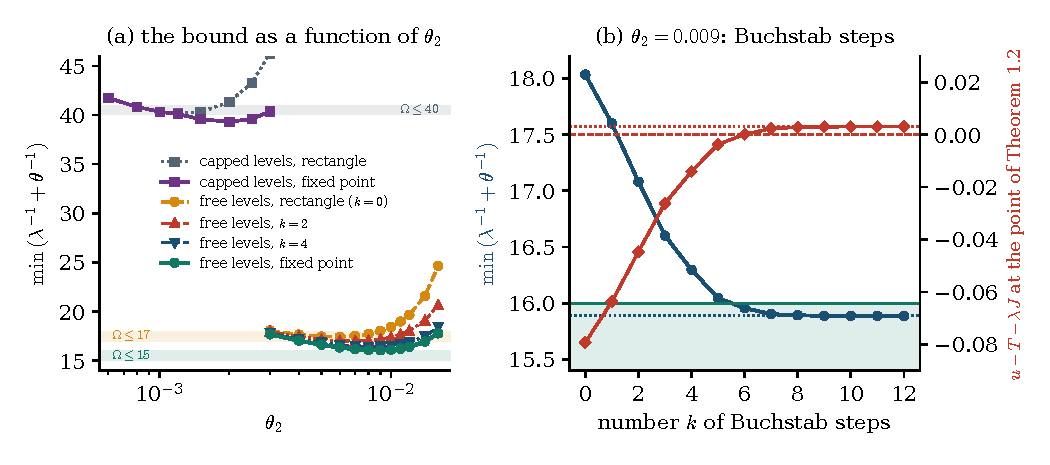
\includegraphics[width=\textwidth]{fig_bound.pdf}
\caption{(a) One-sided values of $\min(\lambda^{-1}+\theta^{-1})$ as a function of $\theta_2$: levels of the
switching step capped as in \cite{NX} or free, rectangle bounds, $k$ Buchstab steps, fixed point; the bands mark
the bounds $40$, $17$ and $15$ (grid $n=800$, $\rho=1.002$; on finer grids the values are lower). (b) At
$\theta_2=0.009$, on the grid of Table~\ref{tab:ksteps}: the minimum after $k$ steps, and $u-T-\lambda J$ at the
point of the proof of Theorem~\ref{thm:15}; the dotted lines are the values at the fixed point.}
\label{fig:bound}
\end{figure}

\begin{figure}[htbp]
\centering
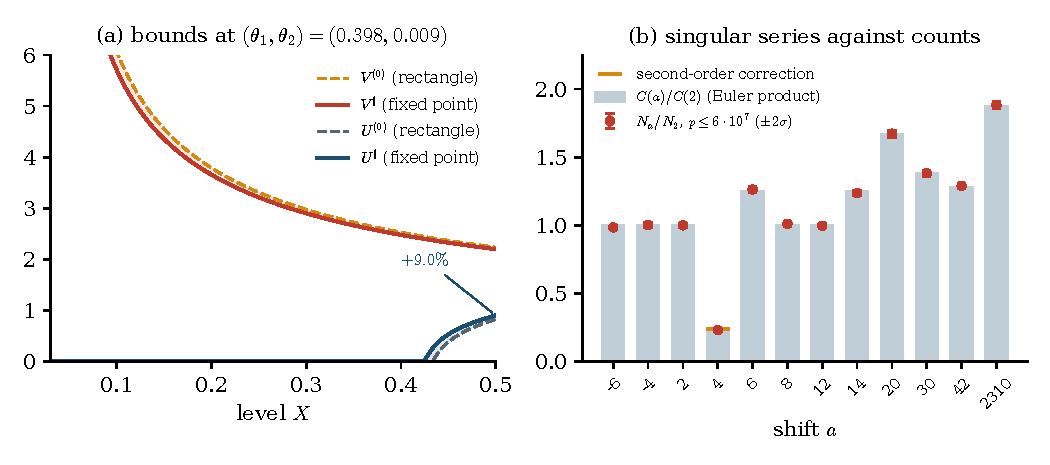
\includegraphics[width=\textwidth]{fig_fixed_point_and_shifts.pdf}
\caption{(a) The tables at $(\theta_1,\theta_2)=(0.398,0.009)$ as functions of the level $X$: rectangle bounds
$U^{(0)},V^{(0)}$ and fixed point $U^\sharp,V^\sharp$ (grid of Table~\ref{tab:ksteps}, on which the gain at
$X=\frac12$ is $9.0\%$). (b) The singular series
$C(a)/C(2)$ of Remark~\ref{rem:counts} against the ratios of the counts up to $6\cdot10^7$; for $a=4$ the mark is
the prediction with the factor $(\log(x/2)/\log(x/18))^{1/2}$ that accounts for the condition on $(p-1)/9$.}
\label{fig:shifts}
\end{figure}

\section{General shifts and the proof of Theorem \texorpdfstring{\ref{thm:shift}}{1.3}}\label{sec:shift}

Let $a\ne0$ be even. Sections~\ref{sec:framework}--\ref{sec:buchstab} were written for a general
$a\not\equiv1\pmod 3$: the shift enters only through the densities, that is through $M_\ell(a)$ and
$S_\ell(a)$, and through the bounded number of primes dividing $a(a+1)$, for which the joint density
$h(\ell,\ell)=1/(\ell-1)$ is of the size of $h(\ell,1)$. The vector sieve \cite[Proposition~3.10]{NX} allows this
for finitely many primes (the constant $C_1$ of its axiom (A2) depends on $a$), as it does for $\ell=3$ when
$a=2$. By Corollary~\ref{cor:KA} the criterion of Proposition~\ref{prop:crit} does not involve $a$, and
$A(a)>0$ because $\rho_a(\ell)<\ell$ for all $\ell>2$: for $\ell=3$ this is the assumption $3\mid a(a+1)$. So
Theorems~\ref{thm:17} and~\ref{thm:15} hold for $p+a$ in place of $p+2$.

Let now $a\equiv1\pmod 3$. Then $\rho_a(3)=3$: if $p\equiv2\pmod 3$ then $3\mid p+a$, and if $p\equiv1\pmod 3$ then
$3\mid p-1$. We use the primes with $9\,\|\,p-1$. Let
\[
\cW=\{(p-1,p+a):\ p\le x,\ p\equiv3\!\!\pmod 8,\ p\equiv10\text{ or }19\!\!\pmod{27}\},
\]
and remove the prime $3$ from both sifting sets. For these $p$ we have $p-1=18k$ with $k\equiv1\pmod4$ and
$3\nmid k$, and $p+a\equiv2\pmod 3$. If $k$ has no prime factor $\equiv3\pmod 4$, then $p-1$ is a sum of two
positive squares. By the Chinese remainder theorem the conditions select two of the $\varphi(216)=72$ reduced
classes modulo $216$, so the number of elements of $\cW$ is $\pi(x)/36$ in place of $\pi(x)/4$, and there is no
sifting at $3$; with $M_3(a)=\frac19$ in \eqref{eq:A}, Lemma~\ref{lem:rect} holds as stated. In the switched
term the elements are $p-1=18mp_1p_2$, with $3\nmid mp_1p_2$, so that $p\equiv10$ or $19\pmod{27}$ holds
automatically, and neither $n+1$ nor $n+1+a$ is divisible by $3$. Their number is $\frac19$ of the number of
$2mp_1p_2\le x$; so Proposition~\ref{prop:switch} holds with $S_3(a)=\frac19$. Since $S_3=M_3$,
Corollary~\ref{cor:KA} and Proposition~\ref{prop:crit} hold without change, and so do the proofs of
Theorems~\ref{thm:17} and~\ref{thm:15}. This proves Theorem~\ref{thm:shift}.

\begin{remark}\label{rem:counts}
The singular series $C(a)$ is $C(2)$ times $\prod(\ell-2)/(\ell-3)$ over the primes $\ell\equiv3\pmod 4$,
$\ell>3$, dividing $a(a+1)$, times $\prod(\ell-1)/(\ell-2)$ over the primes $\ell\equiv1\pmod4$ dividing $a$,
and times $\frac29$ if $a\equiv1\pmod3$. For example $C(6)/C(2)=\frac54$, $C(20)/C(2)=\frac53$ and
$C(4)/C(2)=\frac29$. As a check of the local factors we counted the primes $p\le6\cdot10^7$ of the above classes
for which $p-1$ (resp.\ $(p-1)/9$) has no prime factor $\equiv3\pmod 4$ and $p+a$ is prime: the ratios of the
counts for $a=6,14,20,30,42,2310$ to the count $29946$ for $a=2$ are $1.263$, $1.236$, $1.673$, $1.383$,
$1.290$, $1.883$, against $1.250$, $1.250$, $1.667$, $1.381$, $1.281$, $1.876$ for $C(a)/C(2)$, with standard
errors near $0.01$ (computed as $(N_a/N_2)(1/N_a+1/N_2)^{1/2}$, the counts being treated as Poisson variables); for $a=-4,-6,8,12$ the ratios are $1.004$, $0.985$, $1.012$, $0.998$ against $1$
(Figure~\ref{fig:shifts}(b)). We also
verified $S_\ell(a)=M_\ell(a)$ in exact arithmetic for $\ell<200$ and sixteen shifts, computing $S_\ell$ from
\eqref{eq:Sl}.
\end{remark}

\subsection{Two shifts: proof of Theorem \texorpdfstring{\ref{thm:pair}}{1.4}}\label{sec:pair}
Let $a_1\ne a_2$ be even, non-zero and $\not\equiv1\pmod 3$, and let $\cW$ be the set of triples
$(p-1,p+a_1,p+a_2)$ with $p\le x$, $p\equiv3\pmod 8$. We sift $p-1$ by the primes $q\equiv3\pmod 4$ below
$x^{\theta_1}$, as before, and $n=(p+a_1)(p+a_2)$ by all primes below $z_2=x^{\theta_2}$. The second sieve has
dimension $2$: the density of $\ell\mid n$ is $2/(\ell-1)$ for $\ell\nmid a_1a_2(a_1-a_2)$. The pair is covered by
\cite[Proposition~3.10]{NX} with $(\kappa_1,\kappa_2)=(\frac12,2)$. With \eqref{eq:Mtuple} the local factors are
$M_\ell(a_1,a_2)$, which are positive: $\rho(\ell)\le4<\ell$ for $\ell\ge5$, and $\rho(3)=2$ by the assumption on
$a_1,a_2$ modulo $3$. The main term is normalised by $\cN_2=A(a_1,a_2)\,\theta_2^{-2}\,x(\log x)^{-7/2}$, where
$A(a_1,a_2)=\frac14\kappa e^{-5\gamma/2}\prod_\ell M_\ell(a_1,a_2)(1-\frac1\ell)^{-\nu_\ell-1}$.

\emph{Sieve functions.} For dimension $2$ the sifting limit is $\beta=4.8339865967\ldots$, where $\beta-1$ is the
largest zero of $s^3-6s^2+9s-\frac83$, and \cite[Chapter~11]{FI}
\[
F^{(2)}(s)=\frac{A_2}{s^2}\ \ (0<s\le\beta+1),\qquad
f^{(2)}(s)=\frac{2A_2}{s^2}\Bigl[\log(t-1)-\frac1{t-1}\Bigr]_{t=\beta}^{t=s}\ \ (\beta\le s\le\beta+2),
\]
$f^{(2)}=0$ on $(0,\beta]$, continued by $(s^2F^{(2)})^\prime=2sf^{(2)}(s-1)$ and $(s^2f^{(2)})^\prime=2sF^{(2)}(s-1)$,
with $A_2=43.4968874\ldots$. Both constants can be enclosed directly. The cubic increases for $s>3$ and changes
sign in $[\beta-1-10^{-12},\beta-1+10^{-12}]$. And if $(G,g)$ denotes the solution with $A_2$ replaced by $1$, then
$f^{(2)}\le1\le F^{(2)}$ gives $1/G(S)\le A_2\le1/g(S)$ for every $S$; with enclosures of $G,g$ at $S=16$ we obtain
$43.49680<A_2<43.49697$, which is all that is used below. The upper bound of the sieve holds for $s\ge\beta-1$ and the lower bound for $s\ge\beta$. The
rectangle functions are \eqref{eq:Phi0}--\eqref{eq:G0} with $(F_2,f_2)$ replaced by $(F^{(2)},f^{(2)})$ and the
conditions $s_2\ge2$, $s_2\ge1$ by $s_2\ge\beta$, $s_2\ge\beta-1$.

\emph{Weights.} As $n\le(x+|a_1|)(x+|a_2|)$, the weight $w(n)$ of Section~\ref{sec:framework} satisfies
$w(n)\le1-\lambda(\omega(n)-2\theta^{-1})+o(1)$; a prime $q\ge z_2$ divides $n$ for two classes of $p$ modulo $q$,
so the weighted sum is at most $(2J(\theta)+o(1))\cN_2$; and $n$ is squarefree up to $O(x^{1-\theta_2})$
exceptions, because $(p+a_1,p+a_2)$ divides $a_1-a_2$.

\emph{Switched term.} We use a linear sieve of level $D_1$ for the primality of $n^\prime+1$, $n^\prime=2mp_1p_2$, and a
sieve of dimension $2$, of level $z_2^s$ with $s\ge\beta-1$, for $(n^\prime+1+a_1)(n^\prime+1+a_2)$. The proof of
Proposition~\ref{prop:switch} gives the bound
$K(a_1,a_2)\,C(\theta_1)\,e^{-2\gamma}F^{(2)}(s)/(2\theta_2^2(\frac12-s\theta_2))\cdot x(\log x)^{-7/2}$ with
$K(a_1,a_2)=\frac1{2\sqrt\pi}\prod_\ell S_\ell(1-\frac1\ell)^{-5/2}$. Here, for $\ell>2$, $(\ell-1)S_\ell$ is the
number of residues $n^\prime\bmod\ell$ with $\ell\nmid(n^\prime+1)(n^\prime+1+a_1)(n^\prime+1+a_2)$, where $n^\prime\equiv0$ is
admitted only if $\ell\equiv1\pmod 4$ (it then carries the mass $1/(\ell-1)$ of the $m$ divisible by $\ell$, as in
\eqref{eq:Sl}). With $p=n^\prime+1$ these are the residues $p\notin\{0,-a_1,-a_2\}$, and $p\ne1$ if
$\ell\equiv3\pmod 4$; so $S_\ell=M_\ell(a_1,a_2)$, exactly as in Lemma~\ref{lem:local}; the exponents $\nu_\ell+1-\frac52$ are those of Corollary~\ref{cor:KA}, so
$K(a_1,a_2)/A(a_1,a_2)=2e^{5\gamma/2}/\sqrt\pi$, and the switched term is $(T+o(1))\cN_2$ with
\[
T=\frac{C_1}2\cdot\frac{F^{(2)}(s)\,C(\theta_1)}{\frac12-s\theta_2},\qquad s\ge\beta-1 .
\]
So the criterion is $u-T-2\lambda J(\theta)>0$, with $\theta<\frac12-(\beta-1)\theta_2$, and it gives
$\omega(n)<\lambda^{-1}+2\theta^{-1}$.

\emph{Numerical values.} Section~\ref{sec:buchstab} applies without change, the second sieve being a spectator in
Buchstab's identity. On the grid of Table~\ref{tab:ksteps}, with enclosures of $F^{(2)},f^{(2)}$ of width below
$5\cdot10^{-6}$, the one-sided minimum of $\lambda^{-1}+2\theta^{-1}$ is $39.586$ for the rectangle bounds (at
$\theta_2=0.003$) and $37.677$ for the fixed point (at $\theta_2=0.0035$; $37.679$ at $\theta_2=0.004$). These
values are computed in double precision, as those of Table~\ref{tab:ksteps}. For the proof we take
$(\theta_1,\theta_2,\theta,\lambda)=(0.4,\,0.0035,\,0.2,\,0.036)$ and $s=8.17$ in $T$, and repeat the certified
computation of Section~\ref{sec:buchstab} on the grid $n=1600$, $\rho=1.001$, $b_0=0.002$: the closed form of
$s^2g(s)$ on $[\beta,\beta+2]$ is evaluated in interval arithmetic at the nodes, with the enclosure of $\beta$; the
continuation and the numbers $\psi^\pm_{ij}$ use the four operations with outward rounding and the enclosure of
$A_2$; and the recursion is carried out in integers. This gives, for the table $(U^\sharp,V^\sharp)$,
\[
u\ge0.922903,\qquad T\le0.421423,\qquad 2J(\theta)\le13.879482,
\]
so that $u-T-2\lambda J\ge0.0018>0$, while $\lambda^{-1}+2\theta^{-1}=37.778<38$. This proves
Theorem~\ref{thm:pair}. Table~\ref{tab:cert} collects the two certificates; since the criterion is linear in
$\lambda$, each holds for all $\lambda$ up to the value $\lambda_{\max}$ listed there. We verified
$S_\ell=M_\ell$ in exact arithmetic for $\ell<200$ and eight pairs of shifts.

\begin{table}[htbp]
\centering\footnotesize\setlength{\tabcolsep}{3pt}
\begin{tabular}{lccccccc}
\toprule
& $(\theta_1,\theta_2,\theta,\lambda)$ & $s$ & $u\ge$ & $T\le$ & $\kappa J\le$ & margin $\ge$ & $\lambda_{\max}$\\
\midrule
Theorem~\ref{thm:15} ($\kappa=1$) & $(0.398,\,0.009,\,0.19,\,0.0935)$ & $4.42$ & $0.903518$ & $0.447728$ & $4.841603$ & $0.0031$ & $0.09414$\\
Theorem~\ref{thm:pair} ($\kappa=2$) & $(0.4,\,0.0035,\,0.2,\,0.036)$ & $8.17$ & $0.922903$ & $0.421423$ & $13.879482$ & $0.0018$ & $0.03613$\\
\bottomrule
\end{tabular}
\caption{The certified inequalities $u-T-\kappa\lambda J>0$ (integer recursion on the grid $n=1600$, $\rho=1.001$,
$b_0=0.002$; interval arithmetic for $T$ and for the logarithms in $J$). At $\lambda_{\max}$ the values of
$\lambda^{-1}+\kappa\theta^{-1}$ are $15.886$ and $37.678$.}
\label{tab:cert}
\end{table}

\section{The structure of the criterion and the limits of the method}\label{sec:limits}

\subsection{The regime \texorpdfstring{$\theta_1\to\frac12$}{theta1 -> 1/2}}
Put $\delta=1-2\theta_1$. Since $f_1(s)/F_1(s)=\log(\sqrt s+\sqrt{s-1})\sim\sqrt{s-1}$ as $s\to1$, and
$s_1-1\le(\delta-2s_2\theta_2)/(2\theta_1)$ in \eqref{eq:Phi0}, the main term satisfies
$u\le C_1\sqrt{2\delta}\,(1+O(\delta))$, with near equality when $\theta_2/\delta$ is small. In \eqref{eq:CJ},
$\log\frac{1-\beta-\theta_1}{\theta_1}\sim2(\delta-\beta)$, so
\[
C(\theta_1)\sim\frac83\,\delta^{3/2},\qquad T\sim\frac43\,C_1\,w\,\delta^{3/2},\qquad
w=\begin{cases}4\eg=7.12&\text{levels of \cite{NX}},\\ \min_sF_2(s)/(\frac12-s\theta_2)\approx2.13\text{--}2.19&\text{free levels.}\end{cases}
\]
The main term exceeds the switched term only for $\delta<3/(2\sqrt2\,w)$, and the room $u-T$ left for the
weights is largest at $\delta=1/(2\sqrt2\,w)$. With the levels of \cite{NX} this forces $\delta\approx0.05$,
hence, as $2s_2\theta_2<\delta$ with $s_2\ge2$ and in practice $s_2\approx5$, a sifting range
$\theta_2\approx10^{-3}$ for $p+a$. The integral $J$ then grows like $\log(\theta/\theta_2)$, and $\lambda$ is
small. With free levels $w$ is smaller by the factor $3.3$, the optimum moves to $\delta\approx0.2$ and
$\theta_2\approx0.006$, and the bound drops from $40$ to $17$ (Figure~\ref{fig:terms}). The value
$w=2$ would correspond to an upper-bound sieve of level $x^{1/2}$ for the primality of $n+1$ alone; the cost of the
second condition is the difference $w-2$.

\begin{figure}[htbp]
\centering
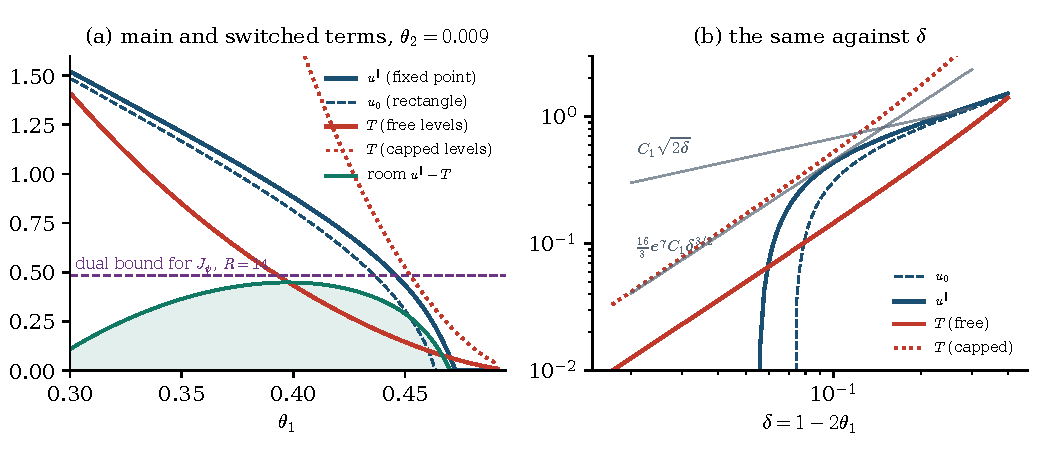
\includegraphics[width=\textwidth]{fig_terms.pdf}
\caption{(a) The main term $u$ (rectangle bound and fixed point), the switched term $T$ (levels capped as in
\cite{NX}, and free), the room $u-T$ for the weights, and the dual bound of Table~\ref{tab:dual} for $R=14$, at
$\theta_2=0.009$. (b) The same on logarithmic scales against $\delta=1-2\theta_1$, with
the asymptotes $C_1\sqrt{2\delta}$ and $\frac{16}3\eg C_1\delta^{3/2}$.}
\label{fig:terms}
\end{figure}

\subsection{The weights}
Consider weights $w_\psi(n)=1-\sum_{q\mid n}\psi(\log q/\log x)$ with a function $\psi\ge0$ on $[\theta_2,1]$. To
conclude $\omega(n)\le R$ from $w_\psi(n)>0$ one needs
\begin{equation}\label{eq:psi-cond}
\psi(\gamma_1)+\dots+\psi(\gamma_{R+1})\ge1\qquad\text{whenever }\gamma_i\ge\theta_2\text{ and }\gamma_1+\dots+\gamma_{R+1}\le1,
\end{equation}
and the criterion becomes $u-T-J_\psi>0$ with $J_\psi=\int\psi(\alpha)v(\frac12-\alpha)\,d\alpha/\alpha$.
Richert's weights are $\psi(\alpha)=\lambda\max(0,1-\alpha/\theta)$ with $\lambda(R+1-\theta^{-1})=1$.

\begin{proposition}\label{prop:richert}
Let $\psi\ge0$ be convex and non-increasing on $[\theta_2,1]$ and satisfy \eqref{eq:psi-cond}, with
$(R+1)\theta_2<1$. Then there are $\lambda$, $\theta$ with $\lambda(R+1-\theta^{-1})=1$ such that
$\psi(\alpha)\ge\lambda\max(0,1-\alpha/\theta)$ on $[\theta_2,1]$. In particular $J_\psi$ is not smaller than the
value of $\lambda J(\theta)$ for these $\lambda$, $\theta$.
\end{proposition}
\begin{proof}
Taking all $\gamma_i=\gamma_0=1/(R+1)$ in \eqref{eq:psi-cond} gives $\psi(\gamma_0)\ge\gamma_0$. Let
$\alpha\mapsto\psi(\gamma_0)-\sigma(\alpha-\gamma_0)$, $\sigma\ge0$, be a supporting line of $\psi$ at $\gamma_0$.
Then $\psi(\alpha)\ge\max(0,\gamma_0-\sigma(\alpha-\gamma_0))$. If $\sigma>0$ the right-hand side is
$\lambda\max(0,1-\alpha/\theta)$ with $\lambda=\gamma_0(1+\sigma)$ and $\theta=\gamma_0(1+\sigma)/\sigma$, and
$\lambda(R+1-\theta^{-1})=(1+\sigma)-\sigma=1$. If $\sigma=0$ then $\psi\ge\gamma_0$ on $[\theta_2,\gamma_0]$,
which exceeds every weight of the family with $\theta\le\gamma_0+\theta_2$ there.
\end{proof}
Without convexity the problem is a linear programme in $\psi$, and its dual gives lower bounds for $J_\psi$ that
hold for every $\psi$. Let $v$ be the step function of Proposition~\ref{prop:uv}, and divide
$[\theta_2,\frac12-\theta_2)$ into cells $I_c$ of length $\Delta$; beyond this range $v=\infty$, so that a $\psi$ with
$J_\psi<\infty$ vanishes almost everywhere there. Call a multiset $\mathbf c=\{c_1,\dots,c_{R+1}\}$ of cells (or of
the symbol $\infty$, for the cell of length $\Delta$ that follows the range) a \emph{configuration} if the right end-points of its
cells sum to at most $1$.

\begin{proposition}[dual bound]\label{prop:dual}
Let $y_{\mathbf c}\ge0$ be weights on finitely many configurations such that
$\sum_{\mathbf c}y_{\mathbf c}\,\#\{m:\ c_m=c\}\le\Delta\inf_{\alpha\in I_c}v(\frac12-\alpha)/\alpha$ for every cell $I_c$. Then
$J_\psi\ge\sum_{\mathbf c}y_{\mathbf c}$ for every measurable $\psi\ge0$ satisfying \eqref{eq:psi-cond}.
\end{proposition}
\begin{proof}
Let $\bar\psi_c$ be the mean of $\psi$ over $I_c$, and $\bar\psi_\infty=0$. For a configuration, every choice of
points $\gamma_m\in I_{c_m}$ is admissible in \eqref{eq:psi-cond}; integrating \eqref{eq:psi-cond} over the product
of the cells gives $\sum_m\bar\psi_{c_m}\ge1$. Hence
$\sum_{\mathbf c}y_{\mathbf c}\le\sum_{\mathbf c}y_{\mathbf c}\sum_m\bar\psi_{c_m}=\sum_c\bar\psi_c\sum_{\mathbf c}y_{\mathbf c}\#\{m:c_m=c\}
\le\sum_c\bar\psi_c\,\Delta\inf_{I_c}v(\frac12-\alpha)/\alpha\le J_\psi$.
\end{proof}
The weights $y_{\mathbf c}$ are found as the dual variables of the linear programme for step functions, solved
with cutting planes (the admissibility of a step function is a knapsack condition), and the hypothesis of the
proposition is then checked directly. With $\Delta=10^{-3}$ and $R=14$ this gives Table~\ref{tab:dual}: for each
$\theta_2$ about $200$ configurations suffice, and the bound exceeds the largest value of $u-T$ over the nodes
$\theta_1\in[0.36,0.43]$ that we examined (every ninth node), even with the smaller $T$ of Section~\ref{sec:sw-buch}. So at these parameters no weight of the
form $w_\psi$, convex or not, gives $\omega(p+a)\le14$ with the tables $u$, $T$, $v$ computed here. This is a
statement about these tables on the parameters examined; it is not an obstruction for a different switching
estimate, a different sieve, or a larger level of distribution. In the other
direction, the optimal step functions have a cost within $0.05\%$ of that of Richert's weights on the same
cells, for $R=15,14,13$: Richert's weights are optimal in this class to the accuracy of the computation.

\begin{table}[htbp]
\centering\small
\begin{tabular}{cccccc}
\toprule
$\theta_2$ & $0.008$ & $0.009$ & $0.010$ & $0.011$ & $0.012$\\
\midrule
$\max_{\theta_1}(u-T)$ & $0.48146$ & $0.46192$ & $0.44168$ & $0.42074$ & $0.39936$\\
dual bound for $J_\psi$, $R=14$ & $0.50413$ & $0.48416$ & $0.46072$ & $0.44428$ & $0.42896$\\
\bottomrule
\end{tabular}
\caption{The dual bound of Proposition~\ref{prop:dual} for $R=14$ against the room $u-T$ (fixed point, grid of
Table~\ref{tab:ksteps}; $T$ with $w^\sharp$).}
\label{tab:dual}
\end{table}
\subsection{The switched term}\label{sec:sw-buch}
The bound $F_2(s_1)F_2(s)$ used in Proposition~\ref{prop:switch} is itself a rectangle bound, for two linear
sieves, and Section~\ref{sec:buchstab} applies to it: Buchstab's identity on the primes $\ell\mid n+1$, with
density $1$ and $V(x^b)\propto b^{-1}$, gives valid upper bounds for the pair, and $F_2(s)/(\frac12-s\theta_2)$
in \eqref{eq:T} may be replaced by $w^\sharp=\min_jV^\sharp_{nj}/C_2$ for the corresponding table. The lower
bounds of the linear sieve vanish for $s\le2$, so that only primes $\ell\le x^{1/6}$ contribute, and the gain is
small: Table~\ref{tab:whatif} lists $w^\sharp$ against the rectangle value $w_0$.

\begin{table}[htbp]
\centering\small
\begin{tabular}{cccc@{\hspace{2.5em}}cc}
\toprule
$\theta_2$ & $w_0$ & $w^\sharp$ & $\min(\lambda^{-1}+\theta^{-1})$ with $w^\sharp$ & $\tau$ & $\min(\lambda^{-1}+\theta^{-1})$ with $\tau T$\\
\midrule
$0.008$ & $2.1691$ & $2.1427$ & $15.787$ & $1.00$ & $15.887$\\
$0.009$ & $2.1901$ & $2.1599$ & $15.743$ & $0.95$ & $15.368$\\
$0.010$ & $2.2112$ & $2.1773$ & $15.761$ & $0.92$ & $15.054$\\
$0.011$ & $2.2325$ & $2.1950$ & $15.834$ & $0.90$ & $14.838$\\
$0.012$ & $2.2539$ & $2.2130$ & $15.964$ & $0.85$ & $14.301$\\
\bottomrule
\end{tabular}
\caption{Left: the switched term with Buchstab's identity on its first sieve, and the resulting one-sided
value (fixed point for $u$ and $J$; grid of Table~\ref{tab:ksteps}). Right: the value that would result if the
switched term were $\tau T$.}
\label{tab:whatif}
\end{table}

The right half of Table~\ref{tab:whatif} shows what the bound would be if the switched term could be reduced
by a factor $\tau$. The bound $14$ requires $\tau\approx0.915$ on this grid, which is almost exactly the limiting value
$\tau=2/w_0\approx0.91$ that corresponds to $w=2$, while Buchstab's identity reaches only $\tau=0.986$. So within the present framework --- vector sieve at the level $x^{1/2}$, switching, weights
of the form $w_\psi$ --- the bound $15$ cannot be lowered by a better treatment of any single ingredient that we
have examined; an improvement would have to come from the switching step, for instance from a level of
distribution beyond $x^{1/2}$ for the switched sequence $\{2mp_1p_2+1\}$.

\subsection*{Data and code}
The repository contains \texttt{code/deep\_sieve\_improvements.py}, whose stages \texttt{level1}, \dots,
\texttt{level4} produce the numbers of Sections~\ref{sec:17}, \ref{sec:buchstab}, \ref{sec:limits} and
\ref{sec:shift}, the stage \texttt{certify} the certificates of Theorems~\ref{thm:15} and~\ref{thm:pair}, and the stage \texttt{pairs}
the numbers of Section~\ref{sec:pair} (outputs in \texttt{data/}), and \texttt{code/make\_acta\_figures.py} for the figures. The
interval arithmetic uses \texttt{mpmath}, the linear programmes \texttt{scipy}; the rest uses \texttt{numpy}.

\subsection*{Acknowledgements}
I thank Kunjakanan Nath and Likun Xie for their correspondence and for coordinating their Erratum with this
paper.

\begin{thebibliography}{99}
\bibitem{FI} J. Friedlander and H. Iwaniec, \emph{Opera de cribro}, Amer. Math. Soc. Colloq. Publ. 57, Amer. Math.
Soc., Providence, RI, 2010.
\bibitem{HBL} D. R. Heath-Brown and X. Li, Almost prime triples and Chen's theorem, J. Number Theory 169 (2016),
265--294.
\bibitem{Iw72} H. Iwaniec, Primes of the type $\varphi(x,y)+A$ where $\varphi$ is a quadratic form, Acta Arith. 21
(1972), 203--234.
\bibitem{Iw76} H. Iwaniec, The half dimensional sieve, Acta Arith. 29 (1976), 69--95.
\bibitem{Iw80} H. Iwaniec, Rosser's sieve, Acta Arith. 36 (1980), 171--202.
\bibitem{Martin} G. Martin, An asymptotic formula for the number of smooth values of a polynomial, J. Number Theory
93 (2002), 108--182.
\bibitem{NX} K. Nath and L. Xie, Almost primes and primes that are sums of two squares plus 1, Acta Arith. 223
(2026), 51--82.
\bibitem{NXerr} K. Nath and L. Xie, Erratum to ``Almost primes and primes that are sums of two squares plus 1'',
Acta Arith., to appear.
\bibitem{Richert} H.-E. Richert, Selberg's sieve with weights, Mathematika 16 (1969), 1--22.
\end{thebibliography}
\end{document}
